\chapter{نمودارهای توالی}

نمودارهای فعالیت مربوط به هریک از موارد کاربرد (با نام مشابه) به تفکیک زیرسیستم در این بخش ارائه می‌شود.

همچنین لازم به ذکر است از ذکر پیش‌نیازها و پس‌نیازها در نمودارهای فعالیت به‌دلیل تطابق کامل آن‌ها با پیش‌نیاز‌ها و پس‌نیازهای جداول توصیف موارد کاربرد صرف‌نظر شد.
\newpage
\section{زیرسیستم کاربری}

\begin{figure}[ht!]
	\centering
	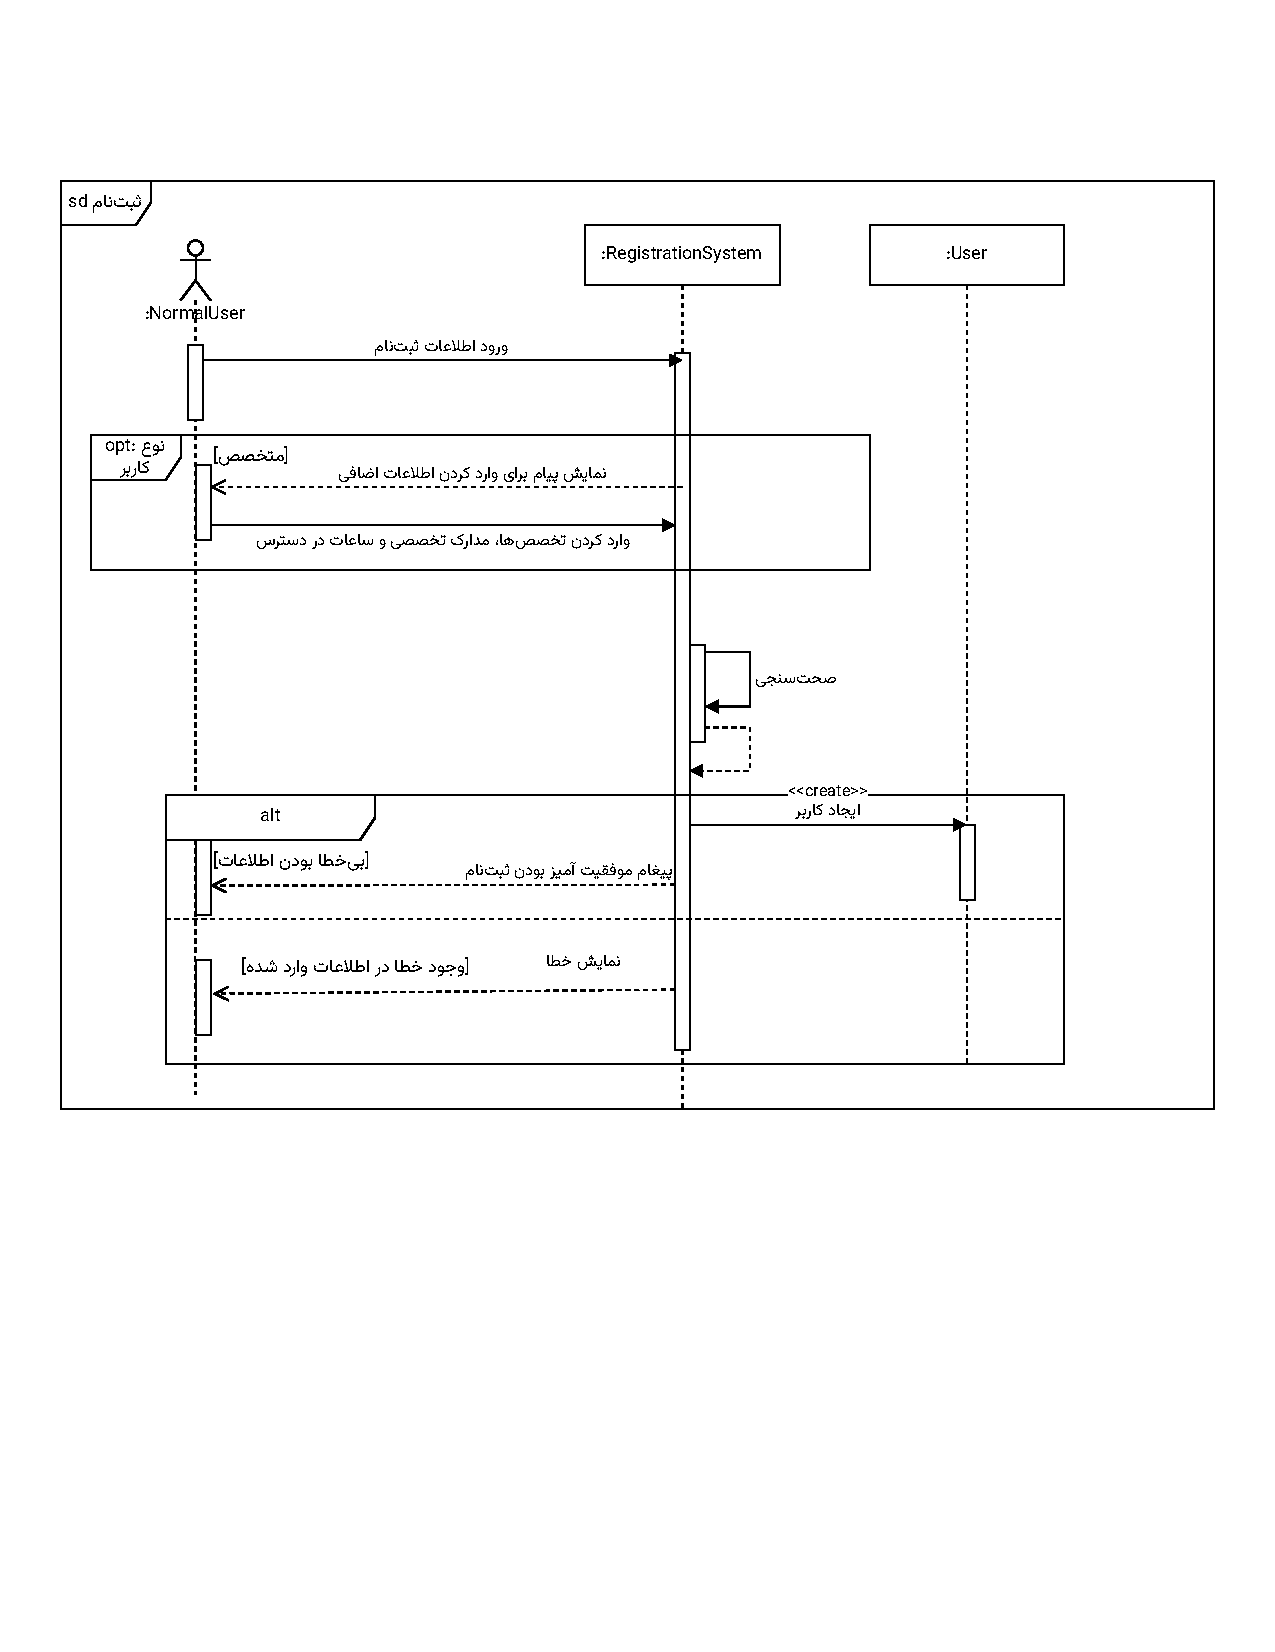
\includegraphics[scale=0.6, page=1]{figs/OOD-Sequence-1.pdf}
	\caption{نمودار توالی: ثبت نام}
\end{figure}
\FloatBarrier
\newpage

\begin{figure}[ht!]
	\centering
	\includegraphics[scale=0.8, page=2]{figs/OOD-Sequence-1.pdf}
	\caption{نمودار توالی: ورود}
\end{figure}
\FloatBarrier
\newpage

\begin{figure}[ht!]
	\centering
	\includegraphics[scale=0.8, page=3]{figs/OOD-Sequence-1.pdf}
	\caption{نمودار توالی: خروج}
\end{figure}
\FloatBarrier
\newpage

\begin{figure}[ht!]
	\centering
	\includegraphics[scale=0.8, page=4]{figs/OOD-Sequence-1.pdf}
	\caption{نمودار توالی: جست‌وجوی کاربران}
\end{figure}
\FloatBarrier
\newpage

\begin{figure}
	\centering
	\includegraphics[scale=0.8, page=5]{figs/OOD-Sequence-1.pdf}
	\caption{نمودار توالی: مشاهده کاربران}
\end{figure}
\FloatBarrier
\newpage

\begin{figure}[ht!]
	\centering
	\includegraphics[scale=0.8, page=6]{figs/OOD-Sequence-1.pdf}
	\caption{نمودار توالی: تایید متخصص}
\end{figure}
\FloatBarrier
\newpage

\begin{figure}[ht!]
	\centering
	\includegraphics[scale=0.8, page=7]{figs/OOD-Sequence-1.pdf}
	\caption{نمودار توالی: اضافه کردن مدیر جدید}
\end{figure}
\FloatBarrier
\newpage

\begin{figure}[ht!]
	\centering
	\includegraphics[scale=0.8, page=8]{figs/OOD-Sequence-1.pdf}
	\caption{نمودار توالی: ویرایش اطلاعات کاربری}
\end{figure}
\FloatBarrier
\newpage


\section{زیرسیستم خدمت‌دهی}


\begin{figure}[ht!]
	\centering
	\includegraphics[scale=0.6, page=9]{figs/OOD-Sequence-1.pdf}
	\caption{نمودار توالی: فیلتر و مرتب‌سازی درخواست‌ها}
\end{figure}
\FloatBarrier
\newpage

\begin{figure}[ht!]
	\centering
	\includegraphics[scale=0.8, page=10]{figs/OOD-Sequence-1.pdf}
	\caption{نمودار توالی: مشاهده درخواست‌ها}
\end{figure}
\FloatBarrier
\newpage

\begin{figure}[ht!]
	\centering
	\includegraphics[scale=0.8, page=11]{figs/OOD-Sequence-1.pdf}
	\caption{نمودار توالی: مشاهده جزئیات درخواست}
\end{figure}
\FloatBarrier
\newpage

\begin{figure}[ht!]
	\centering
	\includegraphics[scale=0.8, page=2]{figs/OOD-Sequence-2.pdf}
	\caption{نمودار توالی: انتخاب متخصص برای خدمت}
\end{figure}
\FloatBarrier
\newpage

\begin{figure}[ht!]
	\centering
	\includegraphics[scale=0.8, page=3]{figs/OOD-Sequence-2.pdf}
	\caption{نمودار توالی: پذیرش درخواست مستقیم مشتری}
\end{figure}
\FloatBarrier
\newpage

\begin{figure}[ht!]
	\centering
	\includegraphics[scale=0.8, page=4]{figs/OOD-Sequence-2.pdf}
	\caption{نمودار توالی: پذیرش درخواست دلخواه}
\end{figure}
\FloatBarrier
\newpage

\begin{figure}[ht!]
	\centering
	\includegraphics[scale=0.8, page=5]{figs/OOD-Sequence-2.pdf}
	\caption{نمودار توالی: پذیرش متخصص}
\end{figure}
\FloatBarrier
\newpage

\begin{figure}[ht!]
	\centering
	\includegraphics[scale=0.8, page=6]{figs/OOD-Sequence-2.pdf}
	\caption{نمودار توالی: لغو درخواست خدمت}
\end{figure}
\FloatBarrier
\newpage

\begin{figure}[ht!]
	\centering
	\includegraphics[scale=0.8, page=7]{figs/OOD-Sequence-2.pdf}
	\caption{نمودار توالی: جست‌وجو و مشاهده متخصصین}
\end{figure}
\FloatBarrier
\newpage

\begin{figure}[ht!]
	\centering
	\includegraphics[scale=0.8, page=8]{figs/OOD-Sequence-2.pdf}
	\caption{نمودار توالی: ثبت درخواست}
\end{figure}
\FloatBarrier
\newpage

\begin{figure}[ht!]
	\centering
	\includegraphics[scale=0.8, page=9]{figs/OOD-Sequence-2.pdf}
	\caption{نمودار توالی: ثبت زمان انجام شدن خدمت}
\end{figure}
\FloatBarrier
\newpage

\begin{figure}[ht!]
	\centering
	\includegraphics[scale=0.8, page=10]{figs/OOD-Sequence-2.pdf}
	\caption{نمودار توالی: ویرایش درخواست}
\end{figure}
\FloatBarrier
\newpage


\section{زیرسیستم بازخورد}


\begin{figure}[ht!]
	\centering
	\includegraphics[scale=0.6, page=11]{figs/OOD-Sequence-2.pdf}
	\caption{نمودار توالی: ارزیابی خدمت دریافت شده}
\end{figure}
\FloatBarrier
\newpage

\begin{figure}[ht!]
	\centering
	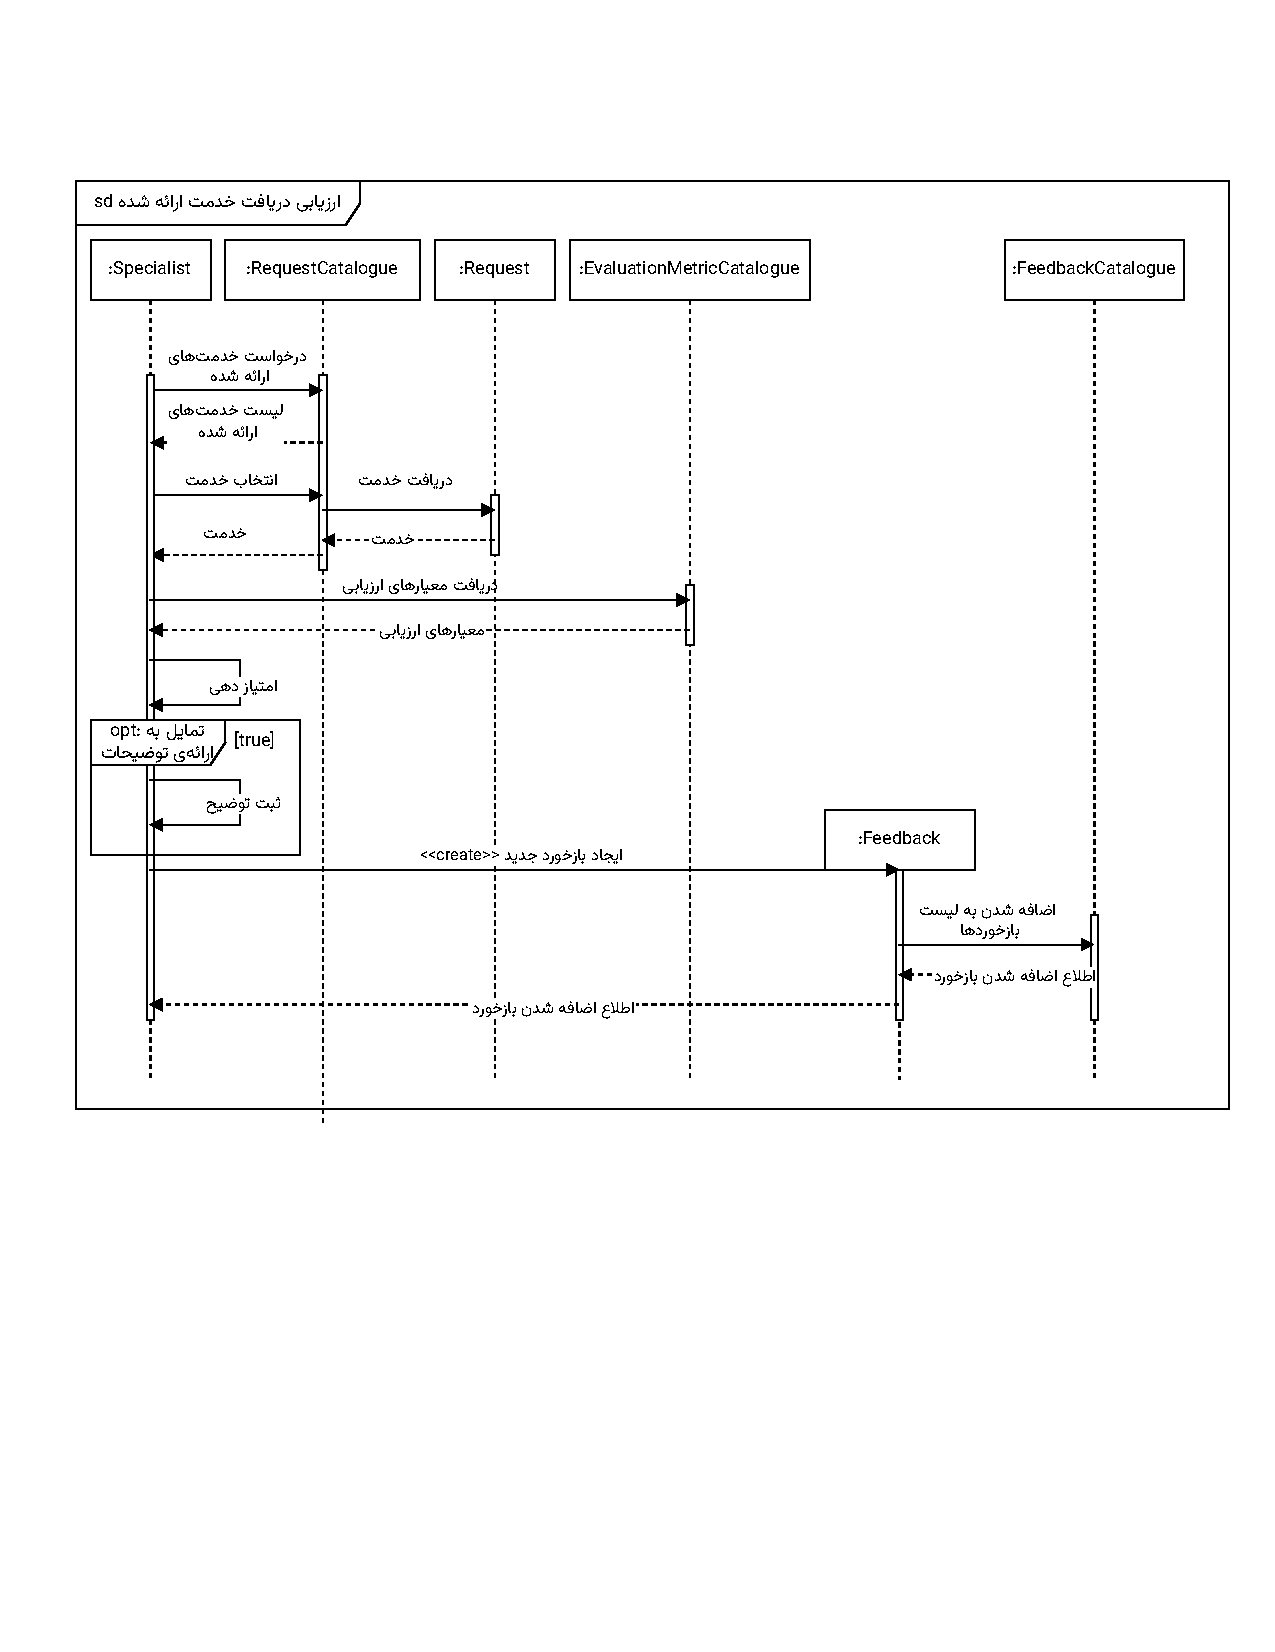
\includegraphics[scale=0.8, page=1]{figs/OOD-Sequence-3.pdf}
	\caption{نمودار توالی: ارزیابی دریافت خدمت ارائه شده}
\end{figure}
\FloatBarrier
\newpage

\begin{figure}[ht!]
	\centering
	\includegraphics[scale=0.8, page=2]{figs/OOD-Sequence-3.pdf}
	\caption{نمودار توالی: مشاهده لیست معیارهای ارزیابی}
\end{figure}
\FloatBarrier
\newpage

\begin{figure}[ht!]
	\centering
	\includegraphics[scale=0.8, page=3]{figs/OOD-Sequence-3.pdf}
	\caption{نمودار توالی: اضافه کردن معیار ارزیابی}
\end{figure}
\FloatBarrier
\newpage

\begin{figure}[ht!]
	\centering
	\includegraphics[scale=0.8, page=4]{figs/OOD-Sequence-3.pdf}
	\caption{نمودار توالی: ویرایش معیار ارزیابی}
\end{figure}
\FloatBarrier
\newpage

\begin{figure}[ht!]
	\centering
	\includegraphics[scale=0.8, page=5]{figs/OOD-Sequence-3.pdf}
	\caption{نمودار توالی: حذف معیار ارزیابی}
\end{figure}
\FloatBarrier
\newpage

\begin{figure}[ht!]
	\centering
	\includegraphics[scale=0.8, page=6]{figs/OOD-Sequence-3.pdf}
	\caption{نمودار توالی: ارسال پیشنهادات و انتقادات}
\end{figure}

\FloatBarrier
\newpage

\section{زیرسیستم مدیریت}
\FloatBarrier
\begin{figure}[ht!]
	\centering
	\includegraphics[scale=0.8, page=7]{figs/OOD-Sequence-3.pdf}
	\caption{نمودار توالی: اضافه کردن امتیاز مورد نیاز برای پذیرش درخواست}
\end{figure}
\FloatBarrier
\newpage


\begin{figure}[ht!]
	\centering
	\includegraphics[scale=0.8, page=8]{figs/OOD-Sequence-3.pdf}
	\caption{نمودار توالی: ویرایش یا حذف امتیاز مورد نیاز برای پذیرش درخواست}
\end{figure}

